\section{Complex numbers}

From the section \hyperref[sec:equations]{Equations} we saw that if the discriminant of a quadratic equation is negative, the
equation has no real solution. For example, the equation $$x^2+4=0$$ has no real solution. If we try to solve this equation, we get $x^2=-4$, so $$x=\pm \sqrt{-4}$$
But this is impossible, since the square of any real number is positive. [For example, $(-2)^2=4$, a positive number.] Thus negative numbers don’t have real square roots.
To make it possible to solve all quadratic equations, mathematicians invented an
expanded number system, called the complex number system. First they defined the new
number $i$ which is, $$i=\sqrt{-1}$$ This means that $i^2=-1$. A complex number is then a number of the form $a+bi$, where $a$ and $b$ are real numbers.

\begin{align*}
    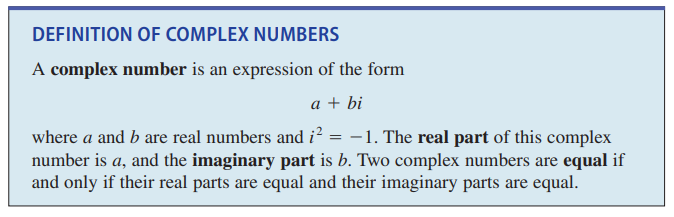
\includegraphics[width=1.1\textwidth]{algebra-pre-calculus/algebra/complex-numbers/complex_numbers_def.png}
\end{align*}

In the complex number the reason why $b$ is being called as the \textbf{imaginary part} is not because it's an imaginary number(when squared produce negative outcome). It's because it's being multiplied by the imaginary number $i$, so it's kind of the "part" of it. The real part is the part that is \textbf{not} being multiplied by $i$. \\

Note that both the real and the imaginary part are real numbers.

A number such as $6i$, which has real part 0, is called a \textbf{pure imaginary number}. A
real number such as $-7$ can be thought of as a complex number with imaginary part 0.
In the complex number system every quadratic equation has solutions. The numbers
$2i$ and $-2i$ are solutions of $x^2-4$ because

\begin{align*}
    (2i)^2  & =4i^2=-4 \\
    (-2i)^2 & =4i^2=-4
\end{align*}

We study complex numbers because they complete, in a useful and elegant
fashion, our study of the solutions of equations. In fact, imaginary numbers are useful not
only in algebra and mathematics, but in the other sciences as well. To give just one example, in electrical theory the reactance of a circuit is a quantity whose measure is an
imaginary number. \\

\subsection{Arithmetic Operations on Complex Numbers}

Complex numbers are added, subtracted, multiplied, and divided just as we would any
number of the form $a+b\sqrt{c}$. The only difference that we need to keep in mind is that $i^2=-1$. Thus the following calculations are valid.

\begin{align*}
    (a+bi)(c+di) & = ac+adi+bci+bdi^2 \\
                 & =ac+(ad+bc)i-bd    \\
                 & = (ac-bd)+(ad+bc)i
\end{align*}

\begin{align*}
    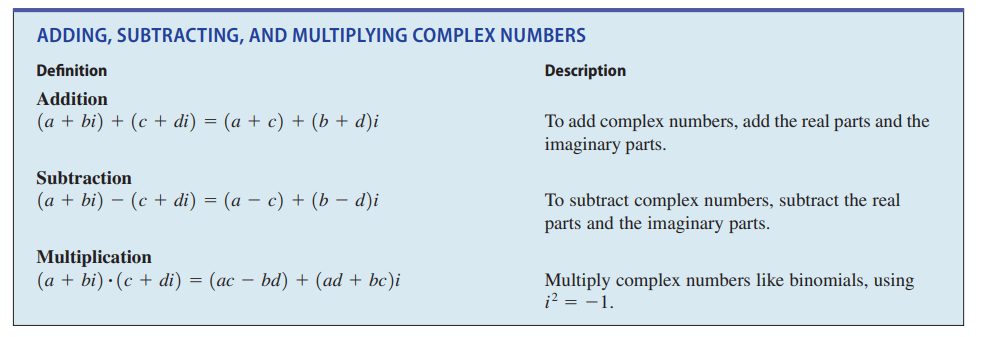
\includegraphics[width=1.1\textwidth]{algebra-pre-calculus/algebra/complex-numbers/arithmetic_operations_complex_numbers.png}
\end{align*}

\subsection{Examples of Adding and subtracting complex numbers}
Express the following complex numbers in the form $a+bi$. \\
\textbf{(a)} $(3+5i)+(4-2i)=(3+4)+(5-2)i=7+3i$ \\
\textbf{(b)} $(3+5i)-(4-2)=(3-4)[5-(-2i)]i=-1+7i$ \\
\textbf{(c)} $(3+5i)(4-2i) = 12-6i+20i-10i^2=12+14i+10=22+14i$ \\
\textbf{(d)} $i^{23}=i^{22+1}=(i^2)^{11}i=(-1)^{11}i=-i$ \\

\subsection{Dividing Complex Numbers}
Division of complex numbers is much like rationalizing the denominator of a radical expression. For the complex number $z=a+bi$ we define its \textbf{complex conjugate} to be the complex number $\overline{z}=a-bi$. The complex conjugate of $z$ is obtained by changing the sign of the imaginary part of $z$. For example, the complex conjugate of $3+5i$ is $3-5i$. \\
Note that, $$z\cdot\overline{z}=(a+bi)(a-bi)=a^2-(bi)^2=a^2+b^2$$
So the product of a complex number and its conjugate is always a nonnegative real number. We use this property to divide complex numbers.

\begin{align*}
    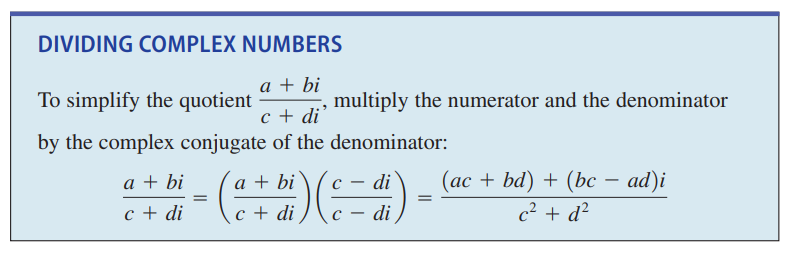
\includegraphics[width=1.1\textwidth]{algebra-pre-calculus/algebra/complex-numbers/dividing_complex_numbers.png}
\end{align*}

Rather than memorizing this entire formula, it is easier to just remember the first step
and then multiply out the numerator and the denominator as usual.

\subsection{Examples of Dividing Complex Numbers}
Express the following complex numbers in the form $a+bi$. \\
\newline
\textbf{(a)} $\displaystyle \frac{3+5i}{4-2i}=\frac{(3+5i)(4+2i)}{(4-2i)(4+2i)}=\frac{22+22i}{20}=\frac{11}{10}+\frac{11}{10}i$ \\
\\
\\
\textbf{(b)} $\displaystyle \frac{7+3i}{4i}=\frac{(7+3i)(-4i)}{(4i)(-4i)}=\frac{-28i-12i^2}{16i^2}=\frac{12-28i}{16}=\frac{3}{4}-\frac{7}{4}i$ \\

\subsection{Square roots of Negative Numbers}
Just as every positive real number $r$ has two square roots ($\sqrt{r}$ and $-\sqrt{r}$), every negative number has two square roots as well. If $-r$ is a negative number, then its square roots are $\pm i\sqrt{r}$ because $$(i\sqrt{r})^2=(-1)(r)=-r$$ and $$(-i\sqrt{r})^2=(-1)(-r)=r$$
\begin{align*}
    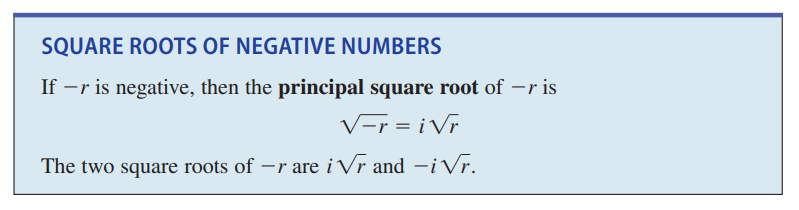
\includegraphics[width=1.1\textwidth]{algebra-pre-calculus/algebra/complex-numbers/square_roots_of_negative_numbers.png}
\end{align*}

There is something that is important to point out. For example if we are trying to find $\sqrt{-16}$ we have two solutions $\pm 4i$. However it's a convention to always consider the \textbf{prinicipal square root} when only one is asked. So in this case we would normally consider the \textbf{prinicipal square root} $\sqrt{-16}=4i$. However both solutions are correct, it is just a convention that we normally follow.
But when we have an equation such as $x^2=-16$ we \textbf{must} provide both solutions, since we have to find \textbf{all} the solutions of the equation. So in this case we would say that $x=\pm 4i$. \\

The second thing to note out is, special care must be taken in performing calculations that involve square roots of negative numbers. Although $\sqrt{a}\cdot\sqrt{b}=\sqrt{ab}$ when $a$ and $b$ are positive, this is not true when $a$ and $b$ are negative. For example, $$\sqrt{-4}\cdot\sqrt{-9}=2i\cdot3i=6i^2=-6$$ but $$\sqrt{(-4)\cdot(-9)}=\sqrt{36}=6 \quad \color{red}\text{Wrong!!} $$
When multiplying radicals of negative numbers, express them first in the form \\ $i\sqrt{r}$ (where $r>0$) to avoid possible errors of this type.

\subsection{Examples of Square roots of Negative Numbers}
Evaluate $(\sqrt{12}-\sqrt{-3})(3+\sqrt{-4})$, expressing your answer in the form $a+bi$. \\
\newline
\textbf{Solution:} \\
\begin{align*}
    (\sqrt{12}-\sqrt{-3})(3+\sqrt{4}) & =(\sqrt{12}-i\sqrt{3})(3+i\sqrt{4})           \\
                                      & =(2\sqrt{3}-i\sqrt{3})(3+2i)                  \\
                                      & =6\sqrt{3}+4i\sqrt{3}-3i\sqrt{3}-2i^2\sqrt{3} \\
                                      & =6\sqrt{3}+i\sqrt{3}+2\sqrt{3}                \\
                                      & =8\sqrt{3}+i\sqrt{3}
\end{align*}


\subsection{Complex Solutions of Quadratic Equations}
We have already seen that if $a\neq0$, then the quadratic equation $ax^2+bx+c=0$ has the solutions, given by the quadratic formula $$x=\frac{-b\pm\sqrt{b^2-4ac}}{2a}$$
If the discriminant $b^2-4ac$ is negative, then the quadratic equation has no real solutions. But it does have complex solutions, because negative numbers have square roots in this expanded setting.

\subsection{Examples of Complex Solutions of Quadratic Equations}
Find the solutions of the following equations. \\
\newline
\textbf{(a)} $x^2+9=0$ \\
\textbf{Solution:} \\
\begin{align*}
    x^2+9 & =0                  \\
    x^2   & =-9                 \\
    x     & =\pm\sqrt{-9}=\pm3i
\end{align*}

\textbf{(b)} $x^2+4x+5=0$ \\
\textbf{Solution:} \\
\begin{align*}
    x^2+4x+5 & =0                                    \\
    x        & =\frac{-4\pm\sqrt{4^2-4(1)(5)}}{2(1)} \\
    x        & =\frac{-4\pm\sqrt{-4}}{2}             \\
    x        & =\frac{-4\pm2i}{2}                    \\
    x        & =-2\pm i
\end{align*}

We see from Example the that if a quadratic equation with real coefficients has complex solutions, then these solutions are complex \textbf{conjugates} (pair of binomials with identical terms but parting opposite arithmetic operators in the middle of these similar terms) of each other. 
So if $a+bi$ is a solutions, then $a-bi$ is also a solution.

\subsection{Complex Conjugate}
First, we need to understand what "conjugate" means in mathematics. 
In general, we can find out the conjugate of an expression by changing the sign in the middle of two terms. 
It only works for expression with two terms(binomials).
E.g: 
\begin{align*}
    \overline{3x+1} & =3x-1 \\
\end{align*}

Such as a number has a conjugate, a complex number also has a conjugate.
It is called complex conjugate.

The complex conjugate of a complex number $z=a+bi$ is the number with an equal real part and an imaginary part equal in magnitude but opposite in sign.
If a and b are real number then the complex conjugate of $a+bi$ is $a-bi$. As we will see later, this skill can be used to divide complex numbers.
If we multiply a complex number by its complex conjugate, the result is a real number in the denominator. 

Denoted: $\overline{z}$



$$\frac{c + di}{a+bi}\cdot \frac{a+bi}{a-bi}$$
Thus, 
$$\frac{(ca + bd) + (ad -cb)i }{a^2 + b^2}$$

As shown above, the denominator is a real number.
If we think graphically, the complex conjugate of a complex number gives us the mirror image of the complex number
about the horizontal axis(real axis).

\subsubsection{Dividing complex numbers}

It is really important to note that dividing by complex numbers with imaginary parts are possible. 
It happens to be more complicated and involves complex analysis. 

$$\frac{2 + 5i}{4 - i}\cdot \frac{4 + i}{4 + i}$$

After expanding it, we get this result: 
$$\frac{3}{17} + \cdot \frac{22i}{17}$$ 
(Note: this is the standard form of a complex number)
To emphasise the denominator's value, we can write in this form:
$$\frac{3+22i}{17}$$
where as we can see the denominator is a real number(17).

\subsection{Complex Conjugates as Solutions of Quadratic Equations}

Show that the solutions of the equation $$4x^2-24x+37=0$$ are complex conjugates of each other. \\
\newline
\textbf{Solution:} \\
\begin{align*}
    x & =\frac{-(-24)\pm\sqrt{(-24)^2-4(4)(37)}}{2(4)} \\
      & =\frac{24\pm\sqrt{-32}}{8}                      \\
      & =\frac{24\pm4i\sqrt{2}}{8}                      \\
      & =\frac{24}{8}\pm\frac{4i\sqrt{2}}{8}            \\
      & =3\pm\frac{1}{2}i\sqrt{2}
\end{align*}
So the solutons are $3+\frac{1}{2}i\sqrt{2}$ and $3-\frac{1}{2}i\sqrt{2}$, which are complex conjugates of each other.